
\begin{fakeXML}[label=kml,caption=A simple KML example representing a Point]
<?xml version="1.0" encoding="UTF-8"?>
<kml xmlns="http://www.opengis.net/kml/2.2">
<document>
<placemark>
  <name>New York City</name>
  <description>New York City</description>
  <point>
    <coordinates>-74.006393,40.714172,0</coordinates>
  </point>
</placemark>
</document>
</kml>
\end{fakeXML} 

\begin{fakeJSON}[label=xml,caption=JSON Data]
\end{fakeJSON} 
\begin{figure}
	\centering
	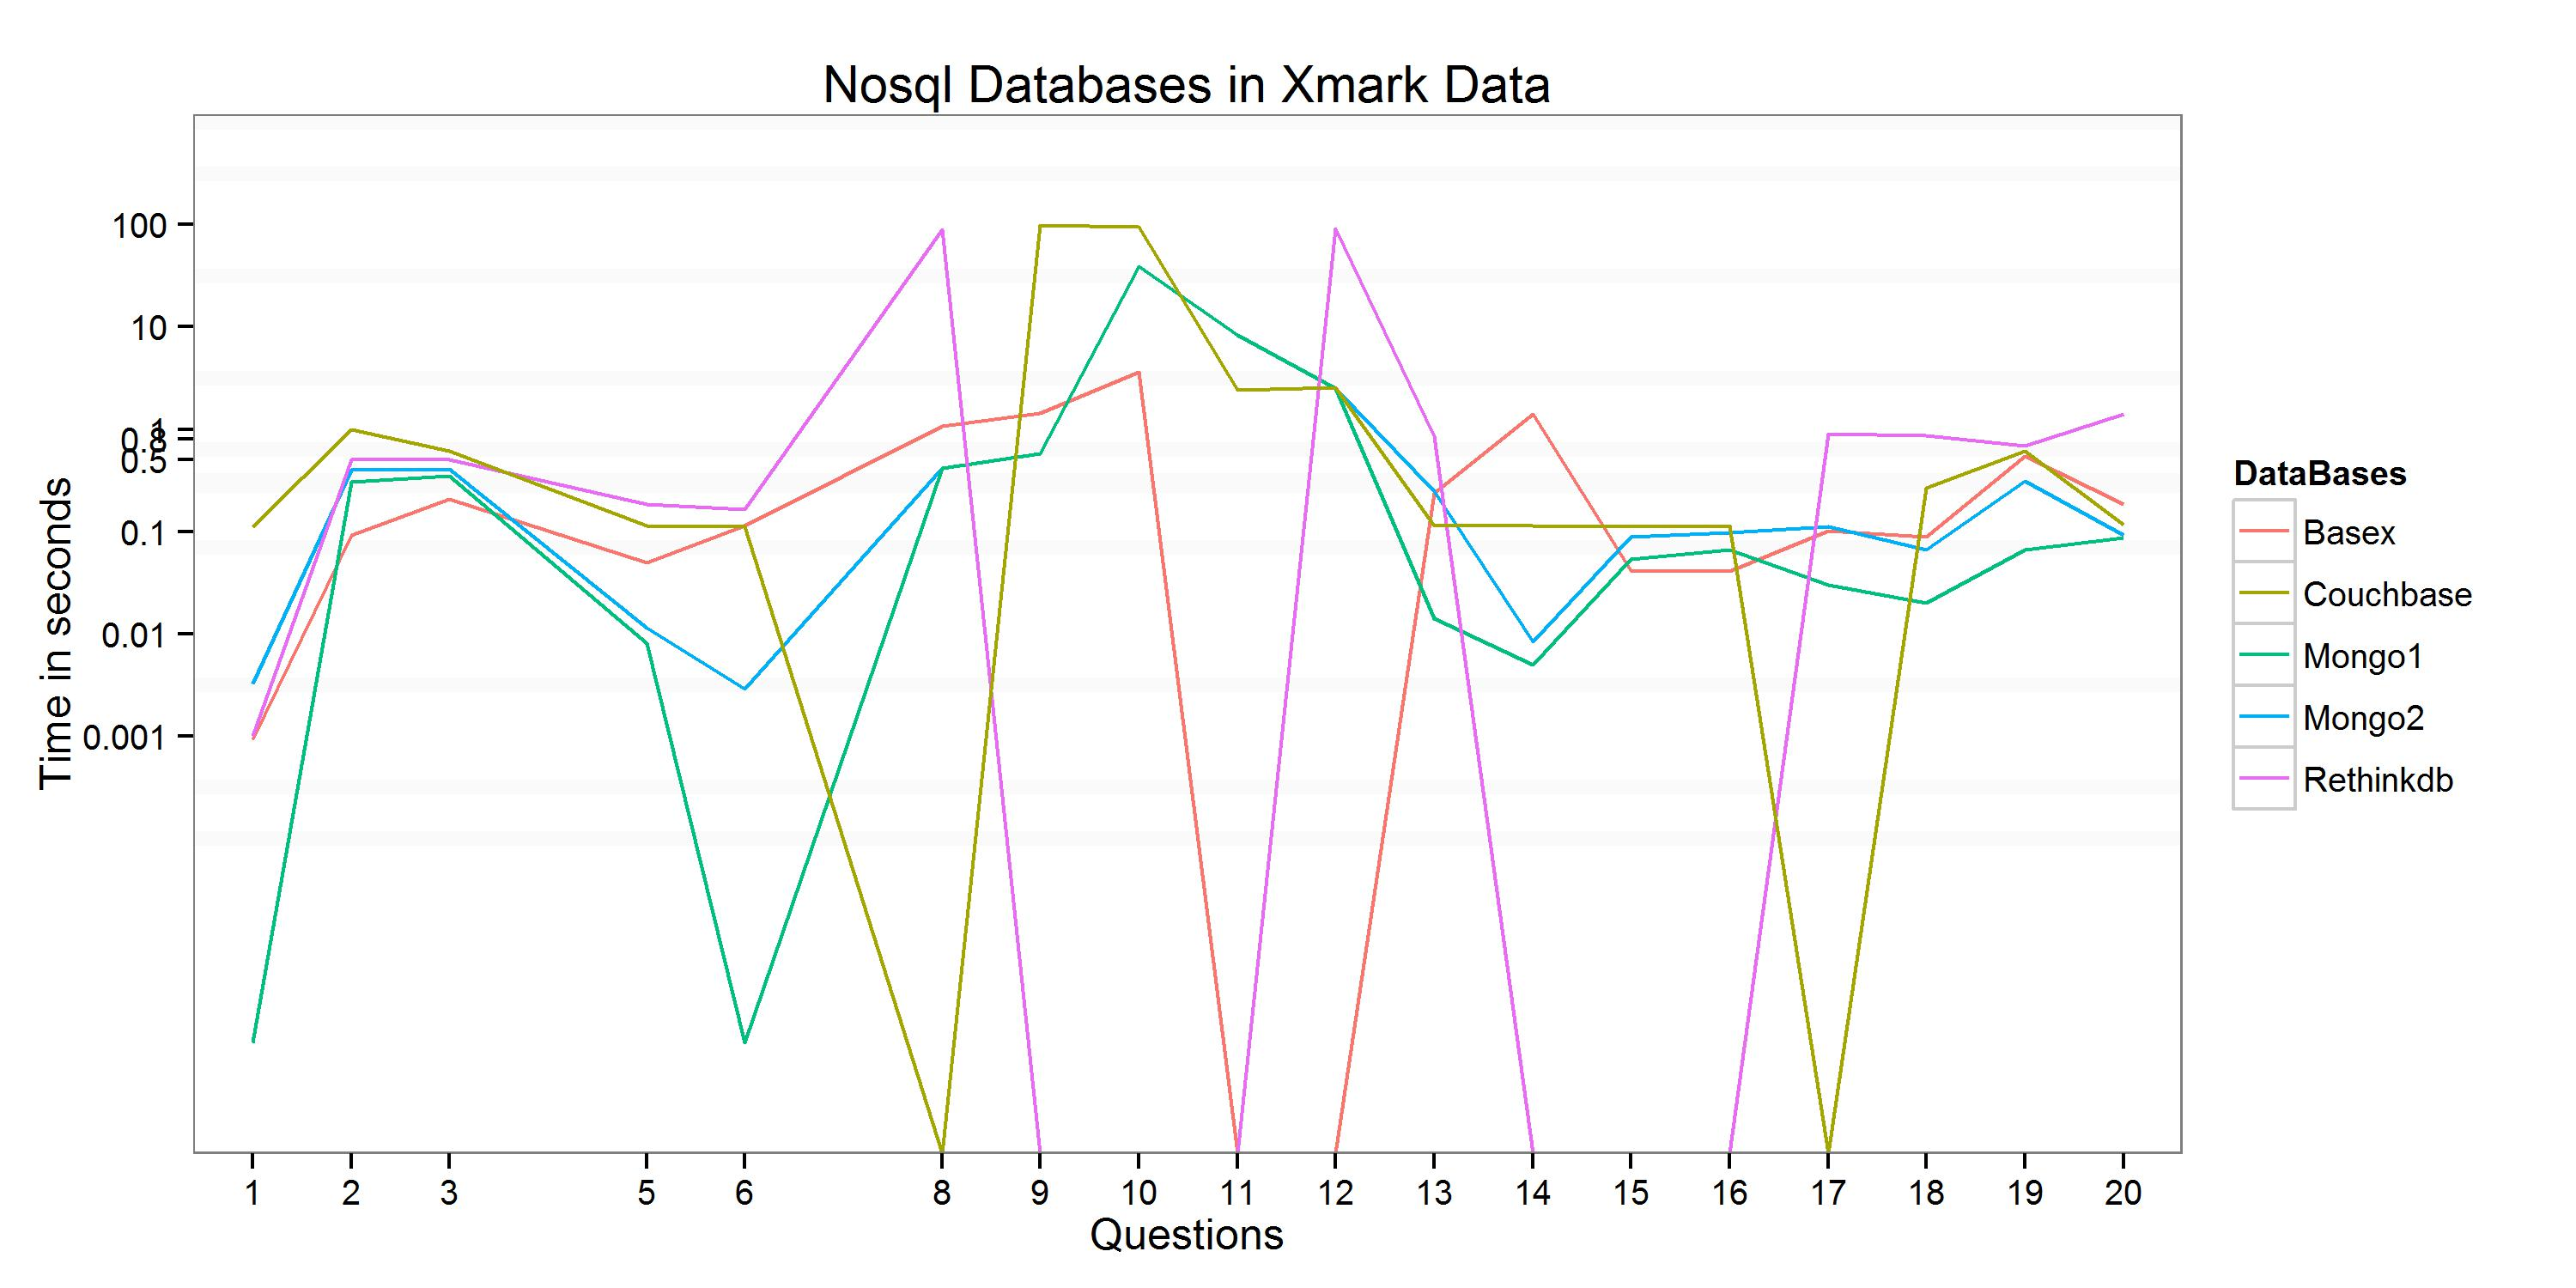
\includegraphics[width=0.9\textwidth]{img/Plot7}
	\caption{An overview of some important indexing structures developed over years}
	\label{trees}
\end{figure}



\begin{lstlisting}
{
"type": "object",
"properties": {
@Name: {
"type": JSON,
"enum": [Fixed]
}
},
required: [@Name]
}
\end{lstlisting}
\begin{minipage}{.5\textwidth}
	\begin{tikzpicture}[%
	grow via three points={one child at (0.5,-0.7) and
		two children at (0.5,-0.7) and (0.5,-1.4)},
	edge from parent path={(\tikzparentnode.south) |- (\tikzchildnode.west)}]
	\node {\{asfdasfd\}}
	child { node [defi] {\textit{Schema\_ID}}}
	child { node [json] {xs:attribute}
		child { node [defi] {\textit{Attribute\_ID}}}
		child { node [attribute] {@name}}
		child { node [attribute] {@type}}
		child { node [attribute] {@fixed}}
		child { node [attribute] {@default}}
	};
	\end{tikzpicture}
\end{minipage}



Mongodb::

Monodbb's collections have a similar and related documents together that helps better indexing ultimately improve in performance. It will not worth to have single collection of whole XMark data as mentioned in \ref{xmark-nosql}. As we shown in Fig.~\ref{fig:xmark-schema}. we create each collection of each substructure in such a way that we will not lose data as well as most representation of xmark data. All sub-structures \textit{items}, \textit{people}, \textit{open\_auctions}, \textit{closed\_auctions}, \textit{catgraph} and \textit{categories} will be collections which store first group entities of XMark mentioned in data~\ref{xmark-dataset} \texttt{item}, \texttt{person},\texttt{open\_auction}, \texttt{closed\_auction} and \texttt{category} as individual documents respectively. In each of these document, one special field \textbf{doctype} is added to represent the value of the parent. for example, in case of person collection \textit{doctype} will be \textit{people}. This key value set will be also the part of document as shoown in Figure~\ref{code:mongodb-person0}. There is one exceptional case in for \textit{item} collection which has \textbf{regions} as grandparent and name of different regions like asia, europe etc. as parent. because of this reason, the \textit{doctype} for item would look like:
\label{code:xmark-mongo-doctype}